\documentclass[conference]{IEEEtran}

\usepackage{amsmath}
\usepackage{amssymb}
\usepackage{booktabs}
\usepackage{cite}
\usepackage{graphicx}
\usepackage{microtype}
\usepackage{url}

\graphicspath{{figures/}}

\title{A Controlled Empirical Study of Tabular Q-Learning and Deep
Q-Network Variants for Cart-Pole Control}

\author{
\IEEEauthorblockN{Chenglin Li}
\IEEEauthorblockA{Participant 006\\Session 1 Robotics Experiments}
}

\begin{document}

\maketitle

\begin{abstract}
Cart-pole balancing is a compact control task that exposes central
reinforcement-learning concepts, including continuous observations, discrete
actions, temporal-difference learning, exploration, and unstable value
estimation. This paper presents a self-contained PyGame-compatible cart-pole
environment and a controlled comparison of tabular Q-learning with deep
Q-network (DQN) variants. Seven learned configurations are trained for an
identical budget of 70,000 environment interactions under three random seeds.
The study varies Q-learning discretization granularity and cumulatively
introduces state normalization, Double DQN targets, and faster exploration
decay to a common DQN implementation. Checkpoints are selected only from a
separate validation set, while development and final evaluation sets contain
disjoint initial-state seeds. On the final set, medium-resolution tabular
Q-learning obtains the strongest result: $490.30\pm9.94$ mean episode steps and
$91.67\%\pm8.39\%$ success. The best DQN configuration by mean performance is
the state-normalized variant, which reaches $472.10\pm48.32$ steps and
$84.33\%\pm27.14\%$ success. Double DQN does not provide a consistent gain
across seeds in this setting. Moreover, every learned method degrades between
its validation-selected best checkpoint and its checkpoint at 70,000 steps,
with substantially larger degradation for the neural agents. These results
show that representation scale, discretization density, repeated trials, and
checkpoint policy can dominate apparently minor implementation choices on a
small control problem.
\end{abstract}

\section{Introduction}

Reinforcement learning (RL) studies how an agent can improve sequential
decisions through interaction. Unlike supervised learning, the desired action
is not supplied at every state. Instead, the agent must connect present
actions to delayed rewards while its own behavior changes the data that it
will observe. Cart-pole balancing is a useful minimal example: a controller
must apply a left or right force to a cart so that a hinged pole remains near
the upright position without moving the cart beyond the track boundary. The
task has been used in early adaptive-control research
\cite{barto1983cartpole} and remains valuable because it has a continuous
state, discrete actions, nonlinear dynamics, and a clear failure condition.

The apparent simplicity of cart-pole can conceal important experimental
questions. A tabular controller requires a finite state representation, so a
continuous observation must be discretized. A DQN avoids explicit
discretization by approximating action values with a neural network
\cite{mnih2015dqn}, but introduces optimization, input scaling, replay-memory,
and target-network choices. Double Q-learning was developed to reduce the
positive bias caused by maximizing noisy value estimates
\cite{hasselt2010double}; its deep variant separates action selection from
target evaluation \cite{vanhasselt2016double}. However, an algorithmic
motivation does not guarantee an improvement on every task or implementation.
Deep RL results can vary substantially across random seeds and experimental
details \cite{henderson2018matters}.

This work therefore treats cart-pole as a controlled empirical study rather
than a demonstration based on one successful run. The following research
questions are considered:

\begin{itemize}
    \item \textbf{RQ1:} How much do state normalization, Double DQN targets,
    and exploration-decay speed change DQN performance?
    \item \textbf{RQ2:} How does state discretization granularity affect
    tabular Q-learning under a fixed interaction budget?
    \item \textbf{RQ3:} Are the learned policies stable across training seeds
    and between the best and final checkpoints?
\end{itemize}

The study makes three practical contributions. First, it implements the
cart-pole dynamics, training algorithms, evaluation protocol, and PyGame
visualization without relying on a prebuilt Gym environment. Second, it
compares four cumulative DQN configurations and three Q-learning
discretizations using the same environment-step budget, three training seeds,
and fixed validation and evaluation seeds. Third, it records both
validation-selected best checkpoints and end-of-budget checkpoints, exposing
training degradation that would be hidden by reporting only the strongest
model. No new RL algorithm is claimed; the contribution is a reproducible,
evidence-driven comparison of design choices.

\section{Background}

\subsection{Markov Decision Process}

The environment is modeled as a Markov decision process
$\langle\mathcal{S},\mathcal{A},P,R,\gamma\rangle$. At time $t$, the agent
observes state $s_t\in\mathcal{S}$, selects action
$a_t\in\mathcal{A}$, receives reward $r_{t+1}$, and observes $s_{t+1}$.
The discounted return is
\begin{equation}
G_t=\sum_{k=0}^{T-t-1}\gamma^k r_{t+k+1},
\end{equation}
where $\gamma\in[0,1)$ controls the importance of future reward. The
action-value function $Q^\pi(s,a)$ is the expected return after selecting
$a$ in $s$ and subsequently following policy $\pi$.

\subsection{Tabular Q-Learning}

Q-learning is an off-policy temporal-difference control method
\cite{watkins1992qlearning}. For a sampled transition
$(s_t,a_t,r_{t+1},s_{t+1})$, its tabular update is
\begin{equation}
\begin{split}
\delta_t &= r_{t+1}+\gamma(1-d_t)
            \max_{a'}Q(s_{t+1},a')-Q(s_t,a_t),\\
Q(s_t,a_t)&\leftarrow Q(s_t,a_t)+\alpha\delta_t,
\end{split}
\label{eq:qlearning}
\end{equation}
where $\alpha$ is the learning rate and $d_t$ indicates termination. The
method is straightforward when every state-action pair can be represented in
a table. For continuous cart-pole observations, each state dimension must
instead be assigned to a finite bin. Coarse bins share experience across a
large region but lose detail; fine bins preserve detail but create a much
larger table whose entries may be visited too rarely.

\subsection{Deep Q-Networks}

DQN replaces the table with a neural approximation
$Q(s,a;\theta)$. The network in this study maps four state values through two
128-unit ReLU layers to two linear action values. It is optimized from
uniformly sampled replay transitions with the smooth L1 loss
\begin{equation}
\mathcal{L}(\theta)=
\operatorname{Huber}\!\left(
Q(s_t,a_t;\theta), y_t
\right),
\end{equation}
where the standard DQN target is
\begin{equation}
y_t=r_{t+1}+\gamma(1-d_t)
\max_{a'}Q(s_{t+1},a';\theta^-).
\label{eq:dqn}
\end{equation}
Here, $\theta^-$ denotes a target network copied periodically from the online
network. Experience replay reduces short-range correlation, and the target
network slows movement of the bootstrap target, two mechanisms central to
the original DQN design \cite{mnih2015dqn}.

In Double DQN, the online network selects the next action while the target
network evaluates it:
\begin{align}
a^*&=\arg\max_{a'}Q(s_{t+1},a';\theta),\\
y_t^{\mathrm{DDQN}}&=r_{t+1}+\gamma(1-d_t)
Q(s_{t+1},a^*;\theta^-).
\label{eq:ddqn}
\end{align}
This separation can reduce maximization bias
\cite{vanhasselt2016double}. DQN still combines function approximation,
bootstrapping, and off-policy updates, a combination associated with value
instability \cite{vanhasselt2018triad}. Target networks can mitigate, but not
eliminate, this interaction \cite{zhang2021target}. Consequently, repeated
training runs and explicit checkpoint rules are necessary for credible
comparison.

\section{Method}

\subsection{Self-Contained Cart-Pole Environment}

The environment state is
\begin{equation}
s_t=[x_t,\dot{x}_t,\theta_t,\dot{\theta}_t]^\top,
\end{equation}
where $x$ is cart position and $\theta$ is pole angle from vertical. The
action space is $\mathcal{A}=\{0,1\}$, corresponding to a force of $-10$ N or
$+10$ N. The simulator uses gravity $9.8$ m/s$^2$, cart mass $1.0$ kg, pole
mass $0.1$ kg, pole half-length $0.5$ m, and a $0.02$ s time step.
Velocities are updated before positions using semi-implicit Euler
integration. At reset, all four state values are sampled uniformly from
$[-0.05,0.05]$.

An episode terminates if $|x|>2.4$ or
$|\theta|>12^\circ$. It succeeds if neither failure occurs for 500 steps.
Each valid transition receives $+1$; failure adds $-10$, while reaching the
500-step limit adds $+10$. Success rate and episode length are therefore more
direct evaluation measures than return, which is nearly determined by
survival time.

\subsection{Tabular Controller}

Position and pole angle are bounded by their termination thresholds.
Velocity and angular velocity are clipped to $[-3,3]$ and $[-3.5,3.5]$,
respectively, before discretization. Three bin vectors are evaluated:
\begin{align*}
\text{Coarse}&=[4,4,8,8],\\
\text{Medium}&=[6,6,12,12],\\
\text{Fine}&=[10,12,20,20].
\end{align*}
The table is updated with \eqref{eq:qlearning}, using
$\alpha=0.2$ and $\gamma=0.99$. The epsilon-greedy exploration rate decays
exponentially from $1.0$ toward $0.03$ according to cumulative environment
steps, with a decay scale of 15,000 steps. Using environment steps rather
than episodes avoids assigning a different exploration schedule merely
because one policy survives longer.

\subsection{DQN Controller}

The online and target networks share a $4$-$128$-$128$-$2$ multilayer
perceptron architecture but hold separate parameters. Hidden layers use ReLU
activation and orthogonal initialization; the output layer uses a smaller
orthogonal gain. The online network is trained with Adam at
$7.5\times10^{-4}$, discount $\gamma=0.99$, batch size 64, a replay capacity
of 50,000 transitions, and gradient-norm clipping at 10. Learning begins
after 500 transitions. The target network is copied every 500 environment
steps.

For normalized variants, each input is divided elementwise by
\begin{equation}
c=[2.4,3.0,0.20944,3.5]^\top.
\end{equation}
This makes the typical scale of all four features comparable. Without this
operation, the pole angle, whose failure boundary is about $0.20944$ radians,
has a substantially smaller numerical range than the translational features.

Table~\ref{tab:dqnvariants} defines the cumulative DQN study. The first three
variants linearly decay epsilon from $1.0$ to $0.05$ over 50,000 steps. The
full variant reaches the same endpoint after 12,000 steps. All other
hyperparameters remain fixed.

\begin{table}[t]
\caption{Cumulative DQN configurations.}
\label{tab:dqnvariants}
\centering
\small
\begin{tabular}{lccc}
\toprule
Variant & Norm. & Double & Decay steps\\
\midrule
Standard DQN & No & No & 50,000\\
Normalized DQN & Yes & No & 50,000\\
Double DQN & Yes & Yes & 50,000\\
Full DQN & Yes & Yes & 12,000\\
\bottomrule
\end{tabular}
\end{table}

\subsection{Checkpoint and Evaluation Protocol}

Each learned configuration is trained independently under seeds 42, 123, and
2026 for exactly 70,000 environment interactions. Validation is performed
every 5,000 steps on 20 episodes beginning at seed 20,000. The checkpoint with
the largest validation mean episode length is named \emph{best}; the model
after the complete budget is named \emph{final}. Only the best checkpoint is
used in the primary comparison, while the difference between best and final
measures late-training degradation.

Two larger evaluation splits are kept separate. Development evaluation uses
100 initial-state seeds from 10,000 through 10,099. These seeds were observed
during implementation and are not treated as unseen test data. Final
evaluation uses seeds 30,000 through 30,099 and was executed only after the
algorithm matrix and checkpoint rule were frozen. Metrics are averaged first
within each 100-episode evaluation and then across the three training seeds.
Reported deviations are sample standard deviations across training seeds,
not standard errors over individual episodes. This convention exposes
run-to-run sensitivity rather than hiding it behind 300 correlated episode
measurements.

\section{Experiments}

\subsection{Experimental Setup}

Training ran on Windows with Python 3.10.19, NumPy 1.26.4, PyTorch
2.6.0+cu124, and an NVIDIA GeForce RTX 4060 Laptop GPU. The complete matrix
contains $7\times3=21$ learned runs and 1,470,000 environment interactions.
A random policy is evaluated under the same episode rules as an untrained
reference. The source tree records a configuration hash, fixed seeds,
checkpoint metadata, per-episode diagnostics, validation curves, and
machine-readable evaluation files.

The primary metrics are mean episode length and the fraction of episodes
reaching 500 steps. Training return, epsilon, and temporal-difference loss are
treated only as diagnostics. This distinction is important because a small
loss does not imply that the greedy policy balances the pole, and return is
almost a linear transformation of episode length in this reward design.

\subsection{Final Performance}

Table~\ref{tab:mainresults} and Fig.~\ref{fig:performance} report final-set
performance for validation-selected best checkpoints. Medium-resolution
Q-learning is strongest on both metrics, obtaining
$490.30\pm9.94$ steps and $91.67\%\pm8.39\%$ success. It exceeds Full DQN by
20.31 mean steps and 12.00 percentage points of success. Coarse Q-learning is
also stable, whereas fine Q-learning has a much larger standard deviation.

\begin{table*}[t]
\caption{Final evaluation of validation-selected best checkpoints. Values are
mean $\pm$ sample standard deviation across three training seeds; each seed is
evaluated for 100 episodes.}
\label{tab:mainresults}
\centering
\small
\begin{tabular}{llrrr}
\toprule
Family & Method & Mean episode length & Success rate & Mean train time (s)\\
\midrule
Reference & Random policy & $20.53\pm1.21$ & $0.00\%\pm0.00\%$ & --\\
\midrule
DQN & Standard DQN & $219.17\pm64.01$ & $0.00\%\pm0.00\%$ & 253.92\\
DQN & Normalized DQN & $472.10\pm48.32$ & $84.33\%\pm27.14\%$ & 378.98\\
DQN & Double DQN & $406.49\pm161.97$ & $72.67\%\pm47.34\%$ & 231.63\\
DQN & Full DQN & $469.99\pm30.58$ & $79.67\%\pm26.27\%$ & 219.75\\
\midrule
Tabular & Q-Learning Coarse & $482.78\pm9.10$ & $82.67\%\pm7.57\%$ & 6.47\\
Tabular & \textbf{Q-Learning Medium} & $\mathbf{490.30\pm9.94}$ &
$\mathbf{91.67\%\pm8.39\%}$ & 6.63\\
Tabular & Q-Learning Fine & $381.90\pm179.87$ & $61.67\%\pm53.69\%$ & 5.79\\
\bottomrule
\end{tabular}
\end{table*}

\begin{figure*}[t]
\centering
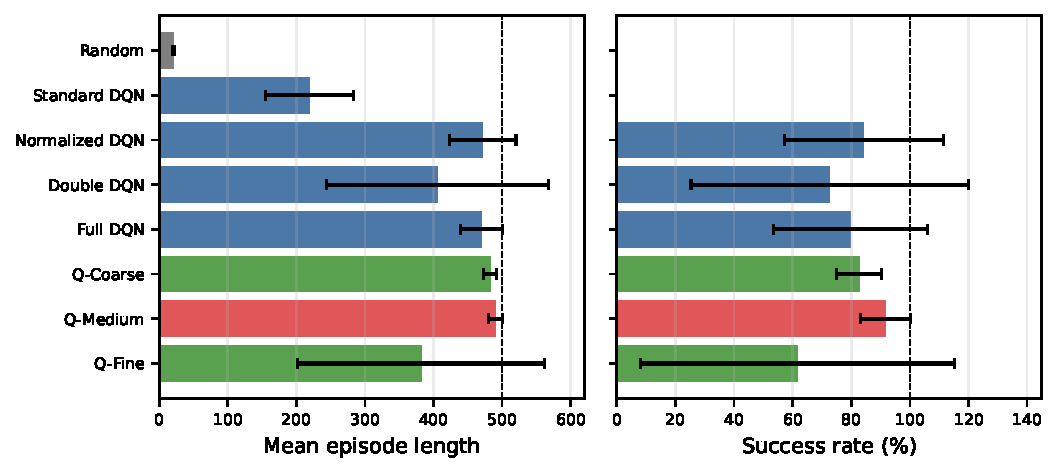
\includegraphics[width=\textwidth]{final_performance.pdf}
\caption{Final-set performance of best checkpoints. Error bars show one
standard deviation across three training seeds. Dashed lines mark the
500-step and 100\% limits.}
\label{fig:performance}
\end{figure*}

\subsection{DQN Ablation: Representation Dominates}

Standard DQN improves substantially over the random policy in episode length
but never reaches the 500-step success criterion. Adding only state
normalization raises mean length by 252.93 steps and success by 84.33
percentage points. This is the largest incremental DQN improvement, answering
RQ1: input scale is critical for this compact MLP and state definition.

Adding Double DQN after normalization does not improve the aggregate result.
Seeds 42 and 2026 both achieve 100\% final-test success with their best
checkpoints, but seed 123 achieves only 18\%. The resulting standard deviation
of 161.97 steps is more than three times that of normalized DQN. Faster
exploration decay in Full DQN recovers mean performance to 469.99 steps and
reduces the episode-length standard deviation to 30.58. Nevertheless,
normalized DQN remains slightly stronger in both mean length and success.
Thus, the experiment supports neither a universal advantage for Double DQN
nor a claim that the cumulative full configuration is best. The intended
reduction of maximization bias addresses one failure mechanism, while
representation and optimization stability remain task dependent.

\subsection{Q-Learning Discretization}

Medium bins provide the best balance between resolution and visitation
frequency, answering RQ2. Coarse discretization is highly repeatable but loses
some control precision: its success ranges from 74\% to 88\% across seeds.
Medium discretization ranges from 82\% to 97\%. Fine discretization performs
well for seeds 42 and 123, at 87\% and 98\%, but fails entirely for seed 2026,
whose best checkpoint reaches only 174.31 mean steps. The fine table therefore
produces $381.90\pm179.87$ steps. Increasing representational capacity without
increasing the interaction budget creates sparse state-action coverage and
can make a seemingly more precise controller less reliable.

\subsection{Checkpoint Degradation}

Figure~\ref{fig:checkpoint} and Table~\ref{tab:checkpoint} answer RQ3. Every
method is weaker at 70,000 steps than at its validation-selected best
checkpoint. The three strongest DQN variants lose approximately 345--352 mean
steps. Tabular methods also degrade, but their mean gaps are 149--179 steps.
The largest DQN collapse is Double DQN, whose final checkpoint averages only
54.56 steps despite a best-checkpoint mean of 406.49.

\begin{figure*}[t]
\centering
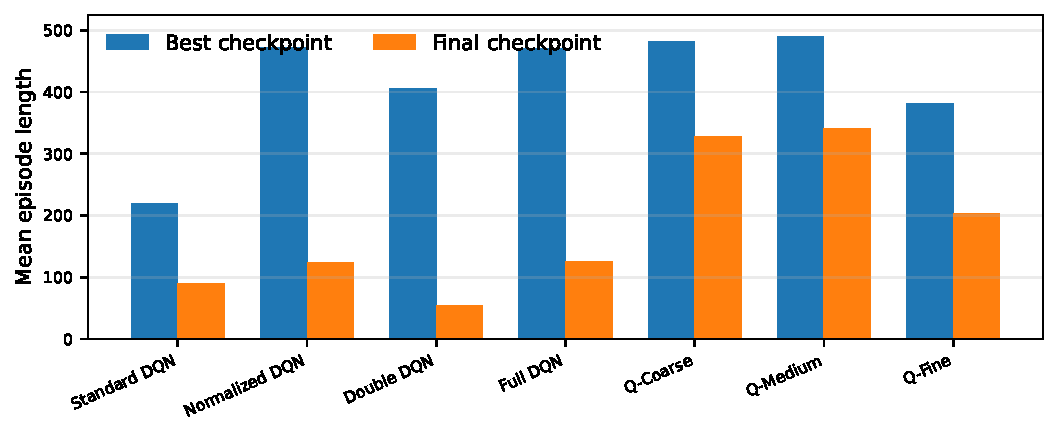
\includegraphics[width=\textwidth]{checkpoint_degradation.pdf}
\caption{Mean final-set episode length for validation-selected best and
70,000-step final checkpoints. Continued training degrades every method.}
\label{fig:checkpoint}
\end{figure*}

\begin{table}[t]
\caption{Best-to-final checkpoint degradation.}
\label{tab:checkpoint}
\centering
\small
\begin{tabular}{lrrr}
\toprule
Method & Best & Final & Gap\\
\midrule
Standard DQN & 219.17 & 90.01 & 129.16\\
Normalized DQN & 472.10 & 124.33 & 347.77\\
Double DQN & 406.49 & 54.56 & 351.92\\
Full DQN & 469.99 & 124.95 & 345.04\\
Q-Coarse & 482.78 & 327.44 & 155.34\\
Q-Medium & 490.30 & 341.33 & 148.97\\
Q-Fine & 381.90 & 202.55 & 179.35\\
\bottomrule
\end{tabular}
\end{table}

The best checkpoint occurs anywhere from 5,000 to 70,000 steps, and its
location varies strongly even within one method. For example, Full DQN is
selected at 65,000 steps for seeds 42 and 123 but at 5,000 steps for seed
2026. The validation curves in Fig.~\ref{fig:curves} are correspondingly
non-monotonic. A fixed end-of-training policy is therefore not a defensible
substitute for validation-based model selection in this experiment.

\begin{figure*}[t]
\centering
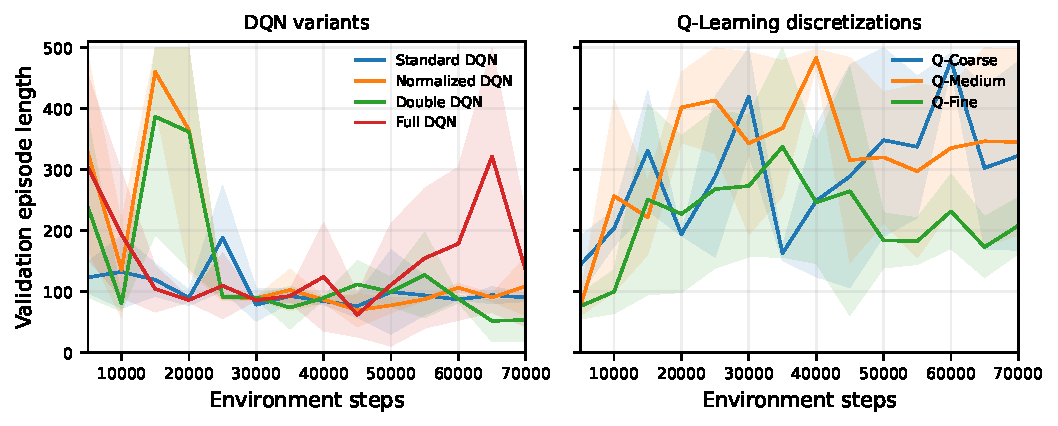
\includegraphics[width=\textwidth]{validation_curves.pdf}
\caption{Validation episode length during training. Lines show the mean over
three training seeds and shaded regions show one standard deviation, clipped
to the valid 0--500 range. Both families exhibit non-monotonic learning.}
\label{fig:curves}
\end{figure*}

The behavior is consistent with known reproducibility concerns in deep RL
\cite{henderson2018matters} and with instability mechanisms that can arise
when off-policy learning, function approximation, and bootstrapping interact
\cite{vanhasselt2018triad}. The tabular agents do not use function
approximation, yet their nonstationary epsilon-greedy data distribution and
constant learning rate can still overwrite useful action values. The result
does not identify one exclusive cause, but demonstrates that a checkpoint
policy materially changes the reported conclusion.

\subsection{Development-to-Test Agreement and Runtime}

The ranking is not an artifact of one evaluation seed range. Across all
learned methods, final-test mean episode length differs from development
evaluation by only $-9.49$ to $+6.74$ steps. Q-Medium changes from
495.33 steps and 94.00\% success on development states to 490.30 and 91.67\%
on final states. Full DQN changes from 475.41 and 81.33\% to 469.99 and
79.67\%. These small shifts support the use of the final values as a
generalization check, while the configuration remains frozen after their
release.

The 21 training records contain 55.16 minutes of accumulated wall-clock time.
Individual DQN runs average 220--379 seconds, compared with approximately six
seconds for a tabular run. These measurements describe this implementation
and hardware rather than theoretical complexity: DQN performs batched
backpropagation at every eligible environment step, whereas Q-learning
updates one table entry.

\subsection{Threats to Validity}

Only three training seeds are available, so the estimated between-run
standard deviations are themselves uncertain. Each checkpoint is selected
from 20 validation episodes, which can favor a noisy local peak. The
500-step horizon causes ceiling effects among strong policies; success rate
is useful but also saturates. Conclusions apply to this self-contained
cart-pole implementation and fixed budget, not automatically to image-based
control or environments with larger action spaces. No confidence interval or
hypothesis test can compensate for the small number of independently trained
agents, so the paper reports effect sizes and individual-seed behavior rather
than claiming statistical significance.

Finally, the cumulative DQN sequence changes one intended factor at each
stage, but the label ``Double DQN'' should not be interpreted as isolating
maximization bias itself; only task performance is observed. Similarly, the
fast exploration schedule is one schedule choice, not a complete exploration
study. These boundaries motivate future work with more training seeds,
learning-rate ablations, larger validation sets, adaptive stopping, and a new
sealed test split if any hyperparameter is changed.

\section{Conclusion}

This paper compared tabular Q-learning and DQN variants for a self-contained
cart-pole control task under a common 70,000-step budget. Medium-resolution
Q-learning delivered the best and most consistent final result. Among neural
agents, state normalization was the decisive modification, while Double DQN
did not yield a consistent cross-seed improvement. Fine tabular
discretization also failed to generalize across training seeds, demonstrating
that additional representational capacity can be counterproductive when
experience is limited.

The strongest lesson is methodological. Every configuration degraded between
its validation-selected best checkpoint and its final checkpoint, and several
DQN policies collapsed after previously solving the task. Reporting one seed
or only the end-of-budget model would therefore produce a misleading account.
Controlled interaction budgets, disjoint evaluation seeds, repeated runs,
and explicit checkpoint selection are not secondary bookkeeping choices;
they determine whether a small RL experiment supports a credible conclusion.

\bibliographystyle{IEEEtran}
\bibliography{references}

\end{document}
